\documentclass[12pt]{article}
\usepackage{amssymb}
\usepackage{amsmath}
\usepackage{amsthm}
\usepackage{array}
\usepackage{graphicx}
  \DeclareGraphicsRule{*}{mps}{*}{}
%\usepackage{bbm}
\usepackage{marvosym}
\usepackage{enumerate}
\usepackage{txfonts}
\usepackage{paralist}
\usepackage{pdfpages}
\usepackage{multicol}
\usepackage{pgfplots}
\pgfplotsset{compat=1.5}
\everymath{\displaystyle}

%\usepackage{showframe}

\pagestyle{empty}

\usepackage{fullpage}
%% \addtolength{\hoffset}{-1.5cm}
%% \addtolength{\textwidth}{3cm}

%% \addtolength{\voffset}{-1.5cm}
%% \addtolength{\textheight}{3cm}

\setdefaultleftmargin{0pt}{}{}{}{}{}

\newcommand{\vv}[2]{#1}

\hyphenpenalty=5000
\tolerance=1000
\setlength{\parindent}{0pt}

\begin{document}

\thispagestyle{empty}
\begin{center}
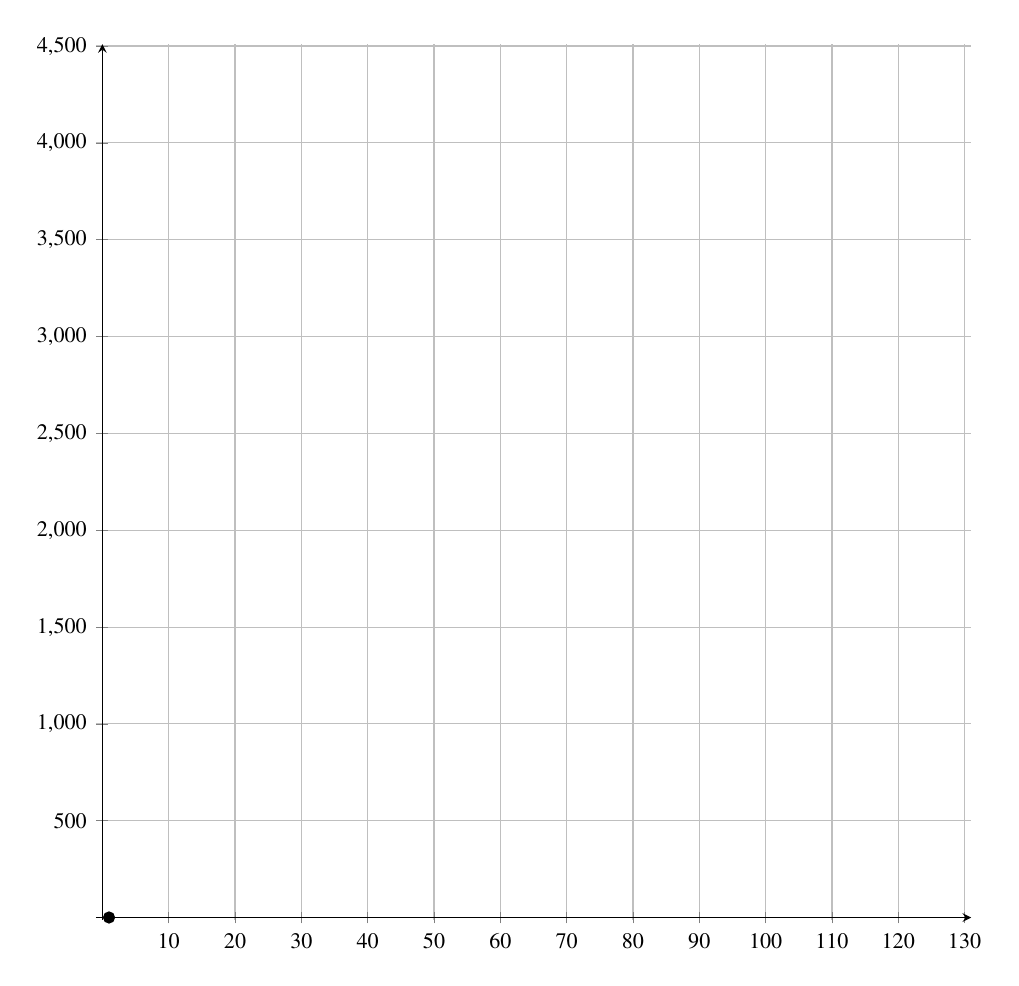
\begin{tikzpicture}
	\begin{axis}[width=5in, height=5in,
		grid=both,
		tick label style={font=\footnotesize},
		xtick distance = 10,
		ytick distance = 500,
		xmin = -1, xmax = 131,
		ymin = -10, ymax = 4510,
		axis x line = middle,
		axis y line = middle,
		]
    \addplot[mark=*] coordinates{(1,0.5)};
	\end{axis}
\end{tikzpicture}
\end{center}

\end{document}
